\chapter{La méthode LATIN}
  
\section{Notations}\label{not_latin}
% ----------------------------

Pour simplifier l'écriture du problème, on introduit les espaces suivants (où $\bullet^*$ désigne les espaces homogènes associés) :\\
\begin{itemize}

\item L'espace $\CA$ des champs $T$ admissibles est comme précédemment :
 \begin{equation}
\mathcal{T} = \{ T \; | \quad T|_{ \bordT} = T_d \quad \textrm{et} \quad T|_{(t=0)} = \Tinit \}
\end{equation}

\item L'espace $\Ad$ des champs solution $(T, \Ys)$ admissibles :
 \begin{equation}
\Ad = \{ (T, \Ys) \; | \quad T \in \CA \quad \textrm{et} \quad  \diver{\Ys}+r = \mvol \capa \frac{\partial T}{\partial t} \quad \textrm{avec} \quad  \Ys  \cdot  \underline{n}|_{ \bordY } = y_d   \}
\end{equation}

\item L'espace $\Comp$ des champs solution $(T, \Ys)$ vérifiant la loi de Fourier :
 \begin{equation}
 \Comp = \left\{ (T, \Ys) \: | \: \underline{Y} = \conduc \:  \gradv{T} \right \}
\end{equation}

\end{itemize}


\section{Stratégie de résolution LATIN avec PGD}


La méthode LATIN (Large Time INcrement method) \cite{Lad85,Lad89,Lad99} a été initialement proposée pour traiter des problèmes non linéaires dépendants  du temps. Depuis son introduction, cette méthode a été exploitée autour de nombreux grands axes de développements :\\
\begin{itemize}
\item Grandes déformations, plasticité (PGD)
\cite{Bussy1984,Vauchez1991,Liu1992}\\

\item Grandes transformations, formulation corotationnelle (PGD)
\cite{Boucard1996b,Michel-Ponnelle2001b}\\

\item Elasto-visco-plasticité, grand nombre de cycles, thermo-élasto-visco-plasticité (PGD)
\cite{Cognard1989,Arzt1994,Cognard1999}\\

\item Dynamique non-linéaire (PGD)
\cite{Royer1990}\\

\item Endommagement et composites\\
\begin{itemize}
\item Formulation fonctionnelle (loi de comportement intégrale) \cite{Allix1992,Guinard2002}
\item Formulation variables internes \cite{Douchin2000b}
\item Multi-échelle composite \cite{Trovalet2010}
\item Couplage flambage-délaminage \cite{Saavedra-Redlich2012b}\\
\end{itemize}

\item Dynamique rapide \cite{Lemoussu2000b,Derumaux2004b,Sen-Gupta2005b}\\

\item Assemblages\\
\begin{itemize}
\item 2D statique \cite{Danwe1993}
\item Evolution vers le 3D (brides en statique) \cite{Champaney1996b}
\item Application en quasi-statique \cite{Blanze2000}
\item Extension à la dynamique \cite{Lemoussu2000b}
\item Optimisation \cite{Boucard10,Laurent2013}\\
\end{itemize}

\item Décomposition de domaine au sens large\\
\begin{itemize}
\item Parallélisme \cite{Ladeveze1987,Lorong1994,Dureisseix1997b}
\item Multiéchelle \cite{Ladeveze1999bb,Loiseau2001b}
\item Multiéchelle - stratégie réutilisation, stochastique \cite{Ladeveze2002}
\item Multiphysique \cite{Dureisseix03}
\item Couplage XFem - fissuration \cite{Guidault2005b}
\item Multiéchelle 3D \cite{Violeau2007b}
\item Multiéchelle temps \cite{Lad10}
\item Amortissement \cite{Caignot2009b}
\item Composites \cite{Kerfriden2008b}\\
\end{itemize}

\item Identification - Problèmes inverses\\
\begin{itemize}
\item Identification avec PGD \cite{Allix2002}
\item Couplage avec RICATI \cite{Nguyen2008}\\
\end{itemize}

\item Multiparamétrique sans PGD\\
\begin{itemize}
\item Assemblages \cite{Boucard03}
\item Dynamique multiéchelle \cite{Odievre2009b}
\item Assemblage composites \cite{Roulet2011d}\\
\end{itemize}

\item Multiparamétrique avec PGD 
\cite{Relun12}\\

\end{itemize}

C'est suivant ce dernier grand axe de recherche que s'illustre cette thèse.\\

De manière très grossière, on peut schématiser la méthode de résolution LATIN comme étant une stratégie qui génère une approximation de la solution $\mathbf{s}$ du problème sur l'ensemble de l'espace et du temps et en améliore automatiquement la qualité à chaque itération, quitte à commencer par une approximation très grossière. En ceci, la méthode est dite non incrémentale.
Cette méthode repose sur 3 principes de base ; la séparation des difficultés, l'approche itérative à 2 étapes et la représentation adaptée des inconnues.\\

%\begin{itemize}
%\item [$\blacktriangleright$] Le point P1 ou la séparation des difficultés \\
%\end {itemize}
  \paragraph{La séparation des difficultés }

Ce point consiste à traiter séparément les difficultés du problème en partitionnant l'espace constitué par l'ensemble des équations que le problème doit vérifier en 2 espaces distincts $\Comp$ et $\Ad$ comme définis en partie \ref{not_latin}. L'espace $\Comp$ est composé des champs vérifiant les équations locales, éventuellement non linéaires (par exemple, pour le problème de diffusion, si la conductivité $\conduc$ dépend de la température $T$), et l'espace $\Ad$ rassemble les champs vérifiant les équations linéaires éventuellement globales.
La solution du problème $\sols_{ref}=(T,\Ys)$ vérifie l'ensemble des équations et se trouve donc à l'intersection de ces 2 espaces : $\sols_{ref} = \Ad \cap \Comp$.\\

%\newpage
%\begin{itemize}
%\item [$\blacktriangleright$] Le point P2 ou l'approche itérative à 2 étapes \\
%\end {itemize}
  \paragraph{L'approche itérative à 2 étapes }

Pour trouver l'intersection de ces 2 espaces, on cherche alternativement une solution de l'un puis l'autre des espaces $\Comp$ et $\Ad$ : la stratégie est donc fondée sur une stratégie itérative à 2 étapes.\\ 


\begin{figure}[!htb]
\centering
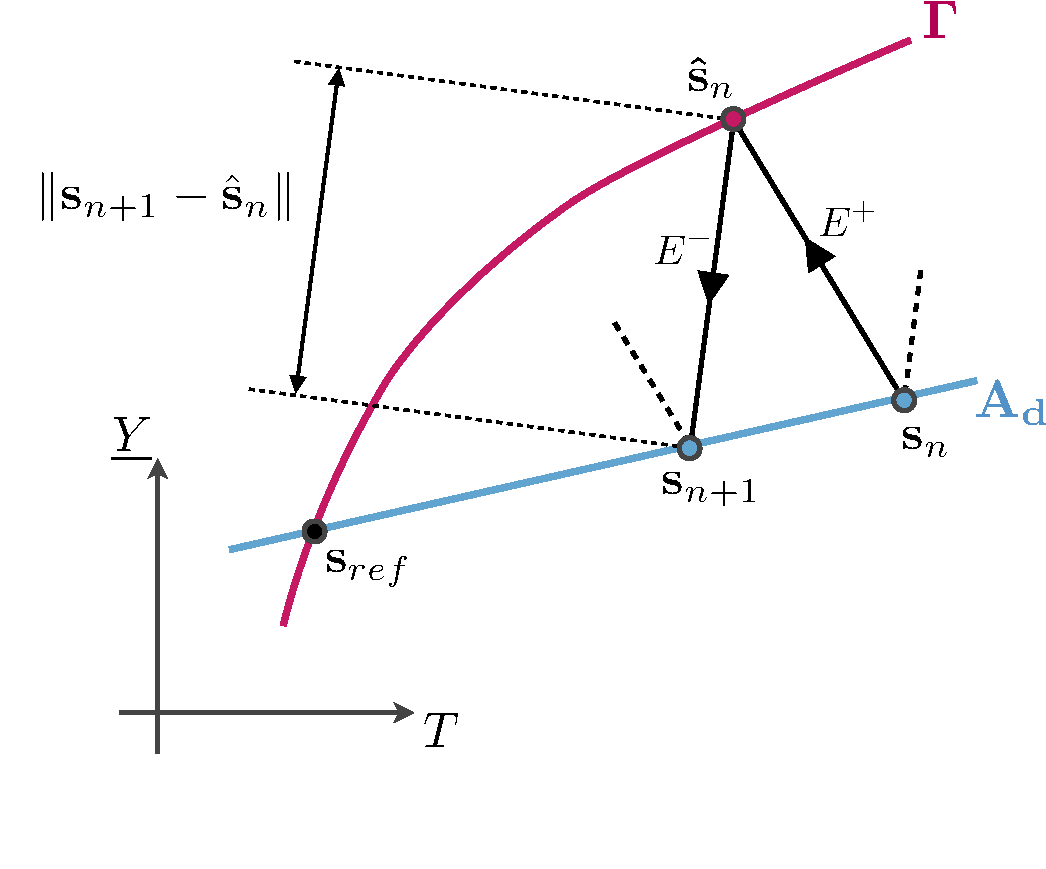
\includegraphics[width=8.8cm]{LATIN.figure/latin_iter_n1}
%\caption{Une itération à l'ordre $n+1$ de la méthode LATIN\label{fig:schema_rom_pgd}}
%\end{figure}
%\begin{figure}[!htb]
\begin{equation}
   \cdots\longrightarrow
   \sols_{n}\in\Ad
   \underbrace{
   \xrightarrow{\text{étape locale}}
   \solsc_{n}\in\Comp
   \xrightarrow{\text{étape linéaire}}
   \sols_{n+1}\in\Ad
   }_\text{iteration $n+1$}
   \longrightarrow
   \solsc_{n+1}
   \longrightarrow\cdots
\end{equation}
\caption{Une itération à l'ordre $n+1$ de la méthode LATIN\label{Latin_schema}}
\end{figure}


Il apparait sur le schéma de la figure \ref{Latin_schema} que l'on doit introduire des \og  directions de recherche\fg{} $\rechp$ et $\rechm$. En effet, le problème complet étant divisé en deux sous-problèmes complémentaires, chacun de ces sous-problèmes manque d'information. Les sous-problèmes n'ont donc pas d'unicité de la solution ou deviennent mal posés et on vient rajouter une équation par cette direction de recherche pour trouver une solution et qu'elle soit unique.\\
 On se donne les directions de recherche $\rechp$ pour l'étape locale et $\rechm$ pour l'étape linéaire (où $h$ est un paramètre de la méthode dont le choix sera détaillé par la suite) :

\begin{equation}\label{dir_rech+}
\rechp:  \quad h\: (\hat{\Ys}_n-\Ys_n)+ (\gradv{\hat{T}_n}-\gradv{T_n}) = 0
\end{equation}
\begin{equation}\label{dir_rech-}
\rechm :  \quad h\: (\Ys_{n+1}-\hat{\Ys}_n)- (\gradv{T}_{n+1}-\gradv{\hat{T}}_n) = 0
\end{equation}\\


Comme schématisé sur la figure \ref{Latin_schema}, l'itération $n+1$ est donc composée :\\
\begin{itemize}
\item d'une étape locale, qui, partant d'une solution connue $\sols_{n} = (T_{n}, \Ys_{n}) \in \Ad$ cherche une solution $\solsc_{n} = (\hat{T}_{n}, \hat{\Ys}_{n}) \in \Comp$ en suivant la direction de recherche $E^+$, \\ 
\item d'une étape linéaire, qui, partant d'une solution connue $\solsc_{n} = (\hat{T}_{n}, \hat{\Ys}_{n}) \in \Comp$ cherche une solution $\sols_{n+1} = (T_{n+1}, \Ys_{n+1}) \in \Ad$ en suivant la direction de recherche $E^-$.\\
\end{itemize}


%\begin{itemize}
%\item [$\blacktriangleright$] Le point P3 ou la représentation adaptée des inconnues \\
%\end {itemize}

    \paragraph{Réduction de modèles }


L'utilisation de la méthode LATIN autour des 2 seuls premiers points suffit à trouver la solution du problème. Cependant la convergence de la méthode est coûteuse avec cette architecture car la solution doit être améliorée à chaque itération sur l'ensemble de l'espace et du temps. En pratique, l'étape locale conduit à la résolution en chaque point d'espace d'un système différentiel en temps (généralement de petite taille) ce qui engendre un coût de calcul modique. En revanche, l'étape linéaire consiste à résoudre un problème global en espace pour chaque pas de temps.\\
La manipulation de la solution sur l'ensemble de l'espace et du temps est donc \textit{a priori} un inconvénient majeur pour le temps de calcul de la stratégie. Cependant, la connaissance de la solution sur $\inttps \times \domaine$ permet de mettre en oeuvre les notions d'approximations spatio-temporelles décrites au chapitre \ref{chapitre2} qui vont en définitive permettre une grande réduction du temps de calcul. C'est donc avec ce troisième aspect que la méthode LATIN prend tout son sens.\\

La PGD permet de calculer l'approximation à variables séparées de la solution sans avoir besoin de réalisations. Elle doit donc être associée à une stratégie permettant de générer à la fois les fonctions du temps et les fonctions spatiales les plus pertinentes pour la solution. De plus, cette stratégie ne peut être incrémentale car chaque couple généré durant le processus doit améliorer l'approximation de la solution sur $\inttps \times \domaine$, ce qui est donc compatible avec la méthode LATIN.\\

Etant donné que le coût de l'étape locale est déjà réduit, on estime que l'introduction de la PGD au cours de cette étape n'aura pas une performance utile et on choisit d'utiliser la représentation PGD uniquement durant l'étape linéaire.\\

L'ajout de la contrainte de représentation sous forme PGD des inconnues rend le problème, déjà constitué des 2 premiers points, sur-contraint. On ne pourra donc pas vérifier l'ensemble des équations. Le but étant ici de réduire le temps de calcul par l'utilisation de la PGD, on impose la représentation PGD des inconnues, et on ne peut ainsi jouer que sur les 2 premiers points de la méthode. Il apparait donc que 2 versions de la méthode LATIN avec PGD sont envisageables :\\

\begin{itemize}
\item Soit en vérifiant \og au mieux\fg{} la direction de recherche. La solution d'une étape s'obtiendra par la résolution d'un problème de minimisation sur l'écart entre la direction de recherche empruntée et celle voulue. On vérifiera donc exactement l'admissibilité de la solution et la représentation PGD. L'idée de cette version peut être schématisée par la figure \ref{rech_au_mieux}.\\
\item Soit en vérifiant \og au mieux\fg{} l'admissibilité de la solution à l'aide d'une approche Galerkin. On vérifiera donc exactement la direction de recherche et la représentation PGD. L'idée de cette version peut être schématisée par la figure \ref{ad_au_mieux}.\\
\end{itemize}
 
 
 
 \begin{figure}[!h]
\begin{center}
\begin{minipage}{5.7cm}
\begin{center}
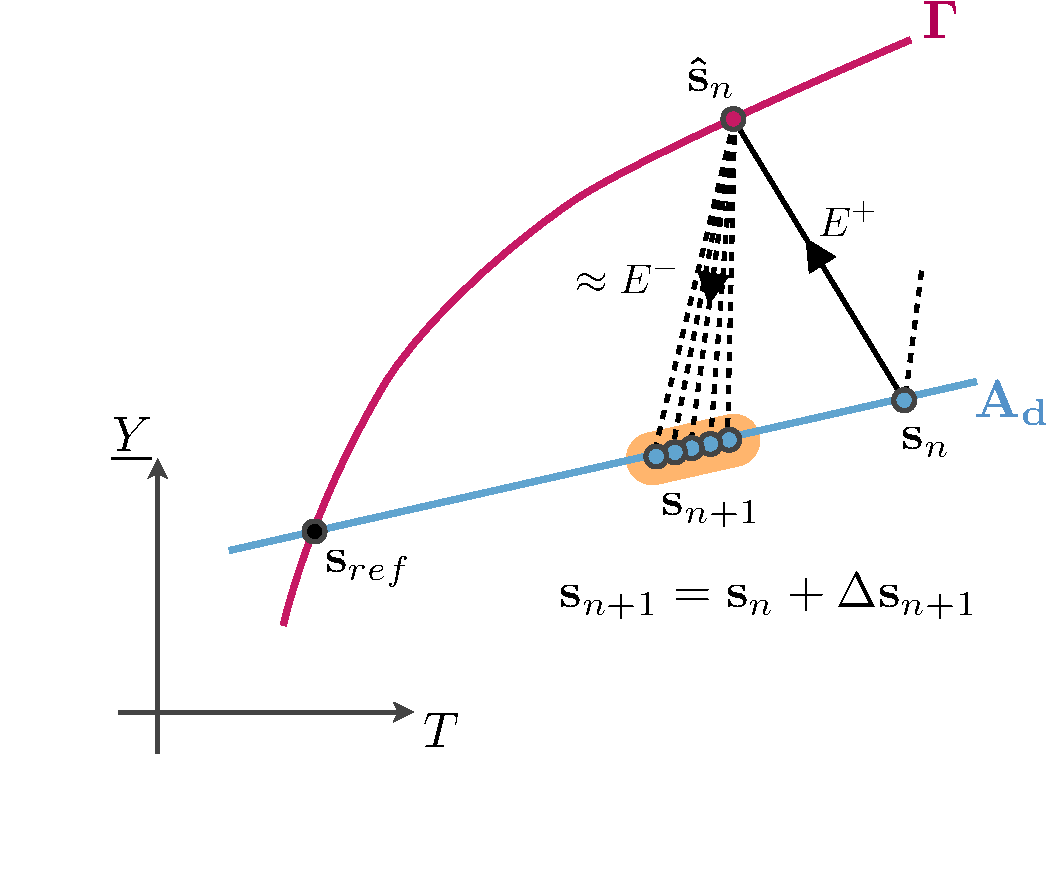
\includegraphics[height=5.45cm]{LATIN.figure/rech_au_mieux}\\
\caption{Vérification au mieux de la direction de recherche\label{rech_au_mieux}}
\end{center}
\end{minipage}%\hfill
\hspace{0.8cm}
\begin{minipage}{5.7cm}
\begin{center}
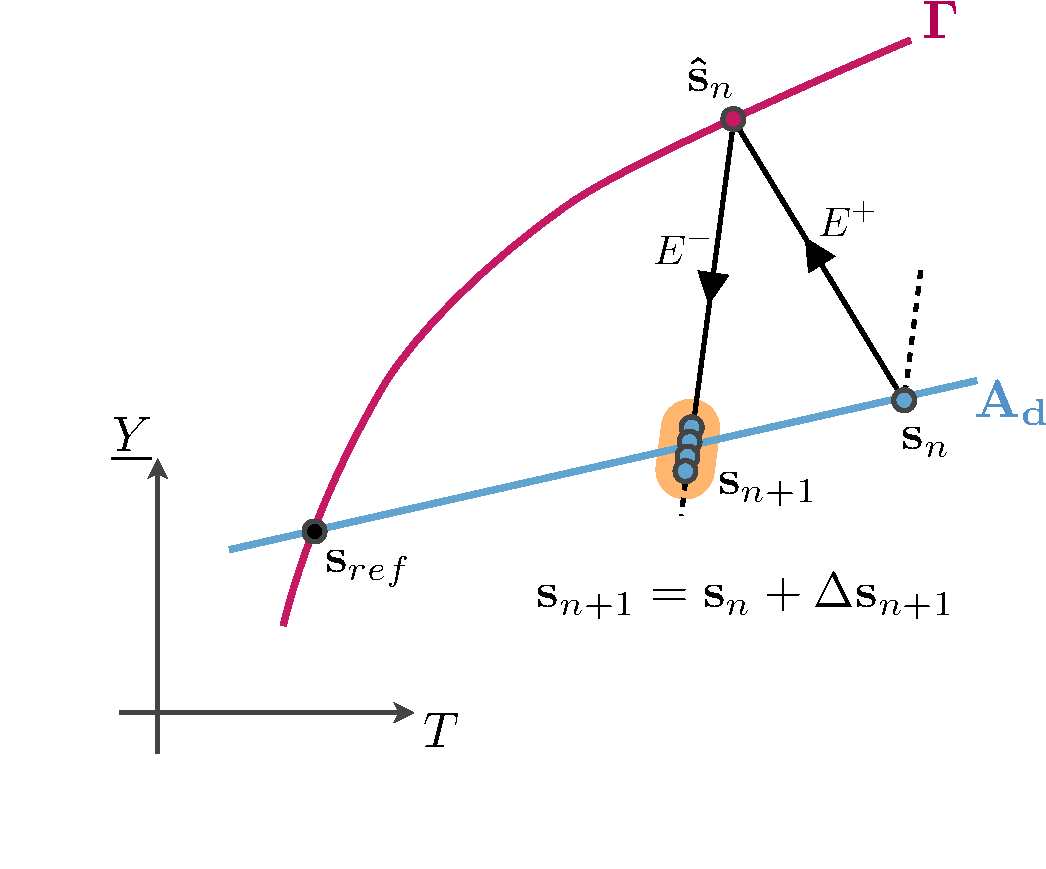
\includegraphics[height=5.45cm]{LATIN.figure/ad_au_mieux}\\
\caption{Admissibilité au mieux de $\sols_{n+1}$\label{ad_au_mieux}}
\end{center}
\end{minipage}
\end{center}
\end{figure}
 
 

 Pour des raisons de simplicité de mise en \oe{}uvre, on choisit de se placer dans le cadre d'une approche Galerkin. Ainsi, on vérifiera exactement la direction de recherche de la méthode ainsi que la représentation PGD de la solution, alors que la solution à chaque itération ne sera admissible qu'au mieux. Cette technique peut parfois mal converger mais ce n'est pas le cas pour le problème ici étudié \cite{Lad10}.\\ 
Etant donné que l'on vérifie exactement la direction de recherche \eqref{dir_rech-}, on peut toujours directement lier $\Ys$ à $T$. On peut donc toujours substituer la variable $\Ys$ par une expression ne dépendant que de $T$. La seule recherche de $T$ sous forme PGD est donc suffisante.\\
Durant l'itération $n+1$, on cherche à améliorer la solution $T_n \in \CA$ à l'aide d'un terme correctif $\Delta T_{n+1} \in \CA^*$. C'est cette correction qui est cherchée sous une forme à variables séparées. 
\begin{equation}
\begin{aligned}
T_{n+1}= T_n + \Delta T_{n+1} \quad \textrm{ où } \quad \Delta T_{n+1} = \tau_{n+1}(t) \: \mathbb{T}_{n+1} (\Ms)
\end{aligned}
\end{equation}
 

  